\oldpage{410}

\begin{figure}[H]
  \centering
  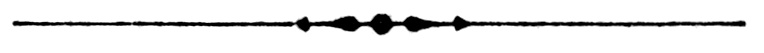
\includegraphics{pages/illustrations/arrow_bullet_divider.jpg}
\end{figure}

\section*{Abortion---The  Medical  Observer and
Its Publisher.}

\byline{Prof.~\ProperName{Cleaveland}}

\SectionStartWords{In the last College Journal} in answering a querie in regard to the
most effectual method of producing abortion, I made some remarks in
regard to a statement published in a medical journal of this city, which
has led to such a curious specimen of \emph{Epistelation} that I am induced
to refer to the matter, and favor the readers of the \ThisJournal{Journal} with the
letter alluded to.

It is well known to the profession in this city that sometime since
\ProperName{Louis Bauer}, \md, of Brooklyn, New York, gave one or more lectures
to the profession, in the Miami Medical College of this city; and that
while here, he was on intimate relations with the editors of the \booktitle{Cincinnati
Medical Observer}.

After his return to the East the \booktitle{Observer}, in March last, published a
communication from him, in which he made some remarks upon the
frequency with which he had been "requested to assist ladies in procuring
abortion." Other circumstances he also stated, which led him to
suppose the production of criminal abortion is of not unfrequent occurrence,
and referred to a lady whose ``death seemed to be connected with
criminal abortion.''   He continued, page 106:

``Since then we have read and heard a good deal of similar instances
and trials in which medical men were implicated, \emph{and in a large city
of the West the medical men with whom we happened to come in
contact, indulged in conversation that led us to the belief that the
procuring of abortion was one of their daily and most lucrative
engagements, in which even men occupying honorable distinction in
the ranks participated}.''

In reference to this charge against members of the profession thus
published and circulated in the \booktitle{Medical Observer}, in my article, I
said:

``Some months since a physician from the East visited this city and
gave one or more lectures, by invitation, before the friends of one of
the Medical Colleges in this city. He was on intimate friendly terms
with the faculty of that College, and after his return to Brooklyn he
published a letter in which he charged upon those with whom he had
associated that their conversation led him to suppose that the unlawful
murder of unborn infants was a common occurrence with them and a
lucrative business.   So far as my personal knowledge of the profession\endinput
